%%  Hello Folks
% chktex-file 1
% chktex-file 2
% chktex-file 8
% chktex-file 24
% chktex-file 32
\documentclass[sigconf, screen, review]{acmart}
% when submitting to PCS change to: \documentclass[sigconf, authordraft, review, anonymous]{acmart}
% when submitting to TAPS change to: \documentclass[sigconf]{acmart}

%% All the added Latex Stuff; packages and new commands.
% ------------------------------------------------
% Packages Etc.
% ------------------------------------------------

% Tables and Formatting
\usepackage{booktabs}
\usepackage{multirow}
\usepackage{multicol}
\usepackage{array} 
\usepackage{makecell} 

% Figures and Wrapping
\usepackage{wrapfig} 
\usepackage{float}
\usepackage[dvipsnames]{xcolor}
\usepackage{enumitem}
\usepackage{graphicx}

% Comments
\usepackage{todonotes}
\newcommand{\cin}{\todo[inline, color=green!80!white!35]}
\usepackage[markup=Highlight,color=pink]{pdfcomment}
\newcommand{\chl}[2][]{\pdfmarkupcomment[author={#1},markup=Highlight]{-- #1 --}{#2}}

% Other
\usepackage{soul}
\usepackage{silence}
\WarningFilter{soulutf8}{This package is obsolete}


% Just for better landmarks when writing
\AtBeginDocument{%
  \hypersetup{
    linkcolor=Green,
    citecolor=Magenta,
    urlcolor=Orange
  }%
}


% ----------------------------------------------

%% \BibTeX command to typeset BibTeX logo in the docs
\AtBeginDocument{%
  \providecommand\BibTeX{{%
    Bib\TeX}}}

%% Rights management information.
%% This information is sent when you complete the rights form.
\setcopyright{acmlicensed}
\copyrightyear{2018}
\acmYear{2018}
\acmDOI{XXXXXXX.XXXXXXX}

%% These commands are for a PROCEEDINGS abstract or paper.
\acmConference[Conference acronym 'XX]{Make sure to enter the correct
  conference title from your rights' confirmation email}{June 03--05,
  2018}{Woodstock, NY}

%% Uncomment \acmBooktitle if the title of the proceedings is different from ``Proceedings of ...''!
%% \acmBooktitle{Woodstock '18: ACM Symposium on Neural Gaze Detection, June 03--05, 2018, Woodstock, NY}
\acmISBN{978--1--4503--XXXX--X/2018/06}

%% Submission ID. -  Use this when submitting an article to a sponsored event.
%%\acmSubmissionID{123-A56-BU3}

%%
%% If you are preparing content for an event sponsored by ACM SIGGRAPH, use "author year" style.
%%\citestyle{acmauthoryear}

%%
\begin{document}
%%

%%
%%[short title in page headers]{Full Title}
\title[shorty]{My Slightly Modified ACM Template: 2025}

%%
%% Only in shared affiliation of the first two authors; "authornote" and "authornotemark"
% \author{Co-First Author}
% \authornote{If two authors contributed equally.}
% \email{number@one.com}
% \orcid{1234-5678-9012}
% \author{Other Co-First}
% \authornotemark[1]
% \email{number@two.com}
% \affiliation{%
%   \institution{University of New Brunswick}
%   \city{Fredericton}
%   \state{New Brunswick}
%   \country{Canada}
%   }
\author{Name}
\orcid{0000--0000--0000--0000}
\email{email@place.ca}
\affiliation{%
	\institution{University of Science}
	\city{Townsville}
	\state{Region}
	\country{area}
}
\author{Name}
\orcid{0000--0000--0000--0000}
\email{email@place.ca}
\affiliation{%
	\institution{University of Science}
	\city{Townsville}
	\state{Region}
	\country{area}
}
\author{Name}
\orcid{0000-0000-0000-0000}
\email{email@place.ca}
\affiliation{%
	\institution{University of Science}
	\city{Townsville}
	\state{Region}
	\country{area}
}

%%
\renewcommand{\shortauthors}{FIRST et al.}

%%
%% ABSTRACT
%%
\begin{abstract}
	\begin{itemize}[label={}, leftmargin=0pt,itemsep=0pt, parsep=0pt] % itemize style i like for short stuff
		\item \textbf{The Way the World Is}
		\item \textbf{The Problem with the World}
			  \par Health, safety, security, happiness, enjoyment, Do things faster / more efficiently / Reduce ``costs'', better understanding, etc.
		\item \textbf{Solution to the Problem (Experiment / System)}
		\item Why it’s a good solution, How to evaluate the solution
		\item \textbf{What We Found Out with Our Study}
		\item \textbf{The Contribution / What We Provided}
	\end{itemize}
\end{abstract}

%%
%% Copy and paste from http://dl.acm.org/ccs.cfm.
%%
\begin{CCSXML}
	<ccs2012>
	<concept>
	<concept_id>00000000.0000000.0000000</concept_id>
	<concept_desc>Do Not Use This Code, Generate the Correct Terms for Your Paper</concept_desc>
	<concept_significance>500</concept_significance>
	</concept>
	<concept>
	<concept_id>00000000.00000000.00000000</concept_id>
	<concept_desc>Do Not Use This Code, Generate the Correct Terms for Your Paper</concept_desc>
	<concept_significance>300</concept_significance>
	</concept>
	<concept>
	<concept_id>00000000.00000000.00000000</concept_id>
	<concept_desc>Do Not Use This Code, Generate the Correct Terms for Your Paper</concept_desc>
	<concept_significance>100</concept_significance>
	</concept>
	<concept>
	<concept_id>00000000.00000000.00000000</concept_id>
	<concept_desc>Do Not Use This Code, Generate the Correct Terms for Your Paper</concept_desc>
	<concept_significance>100</concept_significance>
	</concept>
	</ccs2012>
\end{CCSXML}

\ccsdesc[500]{Do Not Use This Code~Generate the Correct Terms for Your Paper}
\ccsdesc[300]{Do Not Use This Code~Generate the Correct Terms for Your Paper}
\ccsdesc{Do Not Use This Code~Generate the Correct Terms for Your Paper}
\ccsdesc[100]{Do Not Use This Code~Generate the Correct Terms for Your Paper}

%%
%% Keywords that accurately describe the work being presented. Separate the keywords with commas.
\keywords{Do, Not, Use, This, Code, Put, the Correct, Terms, for, Your, Paper}
%% "teaser" image appears typically spans the page.
\begin{teaserfigure}
	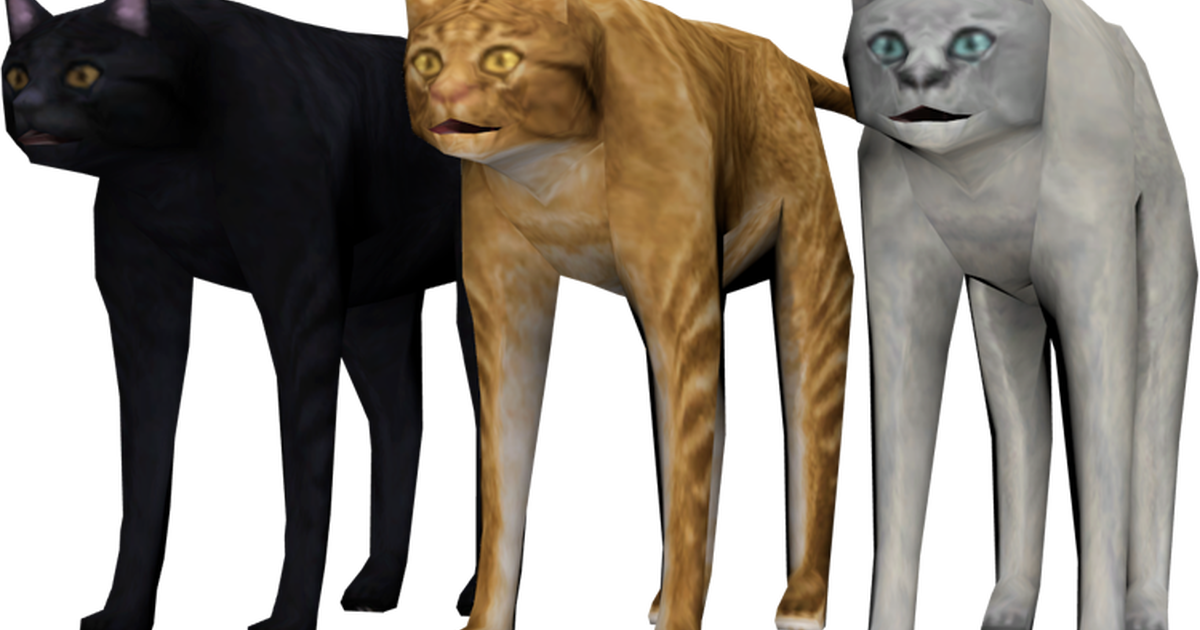
\includegraphics[width=\textwidth]{images/example.png}
	\caption{This is the caption that shows up for the Teaser Image}
	\Description{this is the hidden, secret caption}
	\label{fig:teaser}
\end{teaserfigure}

\received{20 February 2007}
\received[revised]{12 March 2009}
\received[accepted]{5 June 2009}

\maketitle

%%----------------------------------------------
%% Begin Writing Here
%%----------------------------------------------
\section{Introduction}
\par Intro here

\section{Related Work}
\subsection{Nested}
\par Wow. And citation \cite{knuth1990}.
\subsubsection{Nested again}
\par Hmm, same line.

\section{Figure References}
\par (See Figure \ref{fig:testone}), but don't forget figure \ref{fig:testtwo}.

\section{Comments}
\cin{This is a cin comment box}
\par But, we could also do a \chl[klon]{use chl to highlight text} less-flow-breaking comment.

\section{Discussion}
\begin{figure}[!htbp]
	\centering
	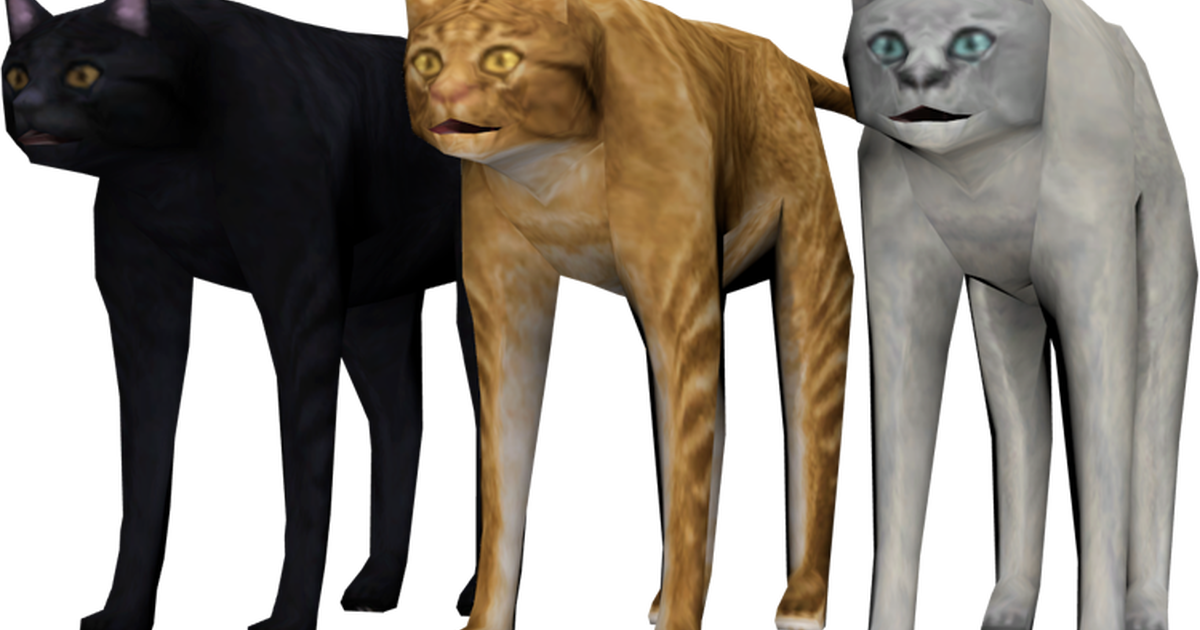
\includegraphics[width=0.85\linewidth]{images/example.png}
	\caption{Single Column image}
	\label{fig:testone}
	\Description{this is the hidden, secret caption}
\end{figure}

\section{Conclusion}
\par Let's wrap it up, but notice spanning figures are tricky to place.\\
See in figure \ref{fig:testtwo} below.
\begin{figure*}[!htbp]
	\centering
	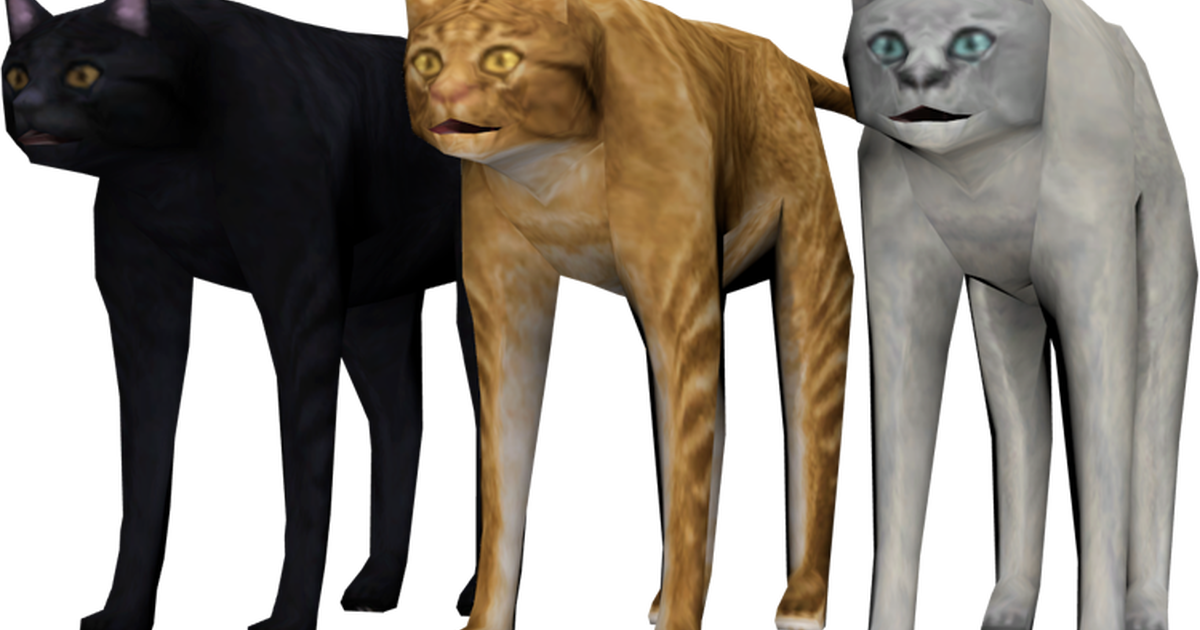
\includegraphics[width=0.7\linewidth]{images/example.png}
	\caption{Double Column image}
	\label{fig:testtwo}
	\Description{this is the hidden, secret caption}
\end{figure*}

\bibliographystyle{ACM-Reference-Format}
\bibliography{bib}
\end{document}
\endinput